\documentclass[pdftex,12pt,letter]{article}
\usepackage[binary-units=true]{siunitx}
\usepackage[margin=0.75in]{geometry}
\usepackage{verbatim}
\usepackage{graphicx}
\usepackage{cite}
\usepackage{color}
\usepackage[pdftex,pdfpagelabels,bookmarks,hyperindex,hyperfigures]{hyperref}
\usepackage{xspace}
\usepackage{amssymb}



\usepackage{tabularx}
\usepackage{url}




\usepackage[firstpage]{draftwatermark}


\bibliographystyle{unsrt}

\newcommand{\fixme}[1]{\textbf{FIXME: #1}}    
\newcommand{\pd}{protoDUNE\xspace}

\title{The protoDUNE-SP experiment and its prompt processing system}
\date{\today}
\author{M.Potekhin for the DUNE Collaboration}

\begin{document}
\SetWatermarkText{DRAFT}
\SetWatermarkLightness{0.9}
\SetWatermarkScale{3}

\maketitle

\begin{abstract}


\noindent The Deep Underground Neutrino Experiment (DUNE) will employ a uniquely large multi-kiloton
Liquid Argon Time Projection Chamber with separate modules utilizing
single and dual-phase Liquid Argon technologies. An experimental 
program (``protoDUNE'')  has been initiated which includes a beam and cosmic ray test of large-scale DUNE prototypes at CERN in 2018.
The volume of data to be collected by the protoDUNE single-phase detector will amount to a few petabytes
and the sustained rate of data sent to mass storage will be in the range of a few hundred megabytes per second.
The protoDUNE experiment requires substantial Data Quality Monitoring capabilities in order to ascertain the
condition of the detector and its various subsystems. To this end, a Prompt Processing system has been deveoped
which is complementary to Online Monitoring and is characterized by a lower bandwidth, scalable CPU resources
and end-to-end latency on the scale of a few minutes. We present the design of the protoDUNE Prompt Processing
system, the current status of its development and testing and issues related to its interfaces and deployment.


\end{abstract}

% \tableofcontents
% \pagebreak

\section{Overview of the protoDUNE-SP}
The \pd program aims to validate various aspects of the DUNE  Liqiud Argon Time Projection Chamber (LArTPC)  technology 
before proceeding with the construction of the large-scale principal DUNE detectors at the Sanford Underground Research
Facility \cite{cdrVol1, cdrVol4}. It  is designed to make a series of measurements of the interactions of
charged particles in the Liquid Argon medium.  These measurements will be performed with a dedicated test
beam  at the CERN SPS accelerator complex and will also include
a large number of cosmic ray triggers. The program includes two separate
large LArTPC prototypes, one based on a ``single-phase'' (liquid) technology and
the other based on a ``dual-phase'' (liquid/gaseous) TPC readout technology.
Both detectors will be placed in an extension of the CERN North Area Experimental Hall.
The general layout of the experimental area is shown in Fig.\,\ref{fig:np02np04}.
Located in this  area will be enclosures which will house the elements of the local computing infrastructure
(including Data Acquisition, Online Buffer etc). These enclosures are shown schematically as yellow blocks in the
upper-right portion of Fig.\,\ref{fig:np02np04}, and they will have a dedicated 20 Gb/s
network connection over optical fiber to the CERN central storage facilities.
% located in the West Area campus of CERN.  

In the following we shall focus on the single-phase prototype which will be referred to as ``protoDUNE-SP''.
It has also received the official CERN designation as the CERN experiment NP04.
This device is essentially an ionization chamber in which Liquid Argon serves both as the target and
the sensitive medium with which to detect and measure ionization, with subsequent full 3D resonstruction of
events of interest. To this end, it is instrumented with a large number
of wire sensors grouped into planar arrays (termed Anode Plane Assemblies, or APAs). Each APA contains
two induction planes and one collection plane, in a stereo angle configuration.

The protoDUNE-SP LArTPC will contain six APAs of the same design as in the DUNE
experiment, and of identical size which is 6$\times$2.4\,m. Drift distance is 3.6\,m
and the drift field 500\,V/cm. The fiducial volume of Liquid Argon in the detector
is approximately 7.2$\times$7.2$\times$6.0\,m$^3$. The cryostat is shaped as a cube
with $\sim$11\,m side (external dimensions).

The detector features the ``cold electronics'' design
in which the amplifiers and digitizers are placed within the cryostat and operate at
cryogenic temperatures. Digital signals are fed to the Warm Interface Boards located
outside of the cryostat and transmitted to the Data Acquisition System via a fiber
optic line.

An important part of the DUNE design is the Photon Detector capable of providing an accurate measurement
of the event timing. It is included in protoDUNE-SP and components of this detector are integrated
into the APAs.

In order to implement the Cosmic Ray Trigger an external system of scintillation counters is installed
outside of the cryostat. The signals from the counters are used in the trigger logic and are also
read out and also included in the overall data stream created by the DAQ.

The beamline used in the experiment is instrumented with fiber tracking devices, Time-of-Flight and Cherenkov counters.
% These detectors are read out separately and their respective data is transmitted to the




%%%%%%%%%%%%%%%%%%%%%%%%
\begin{figure}[tb]
\centering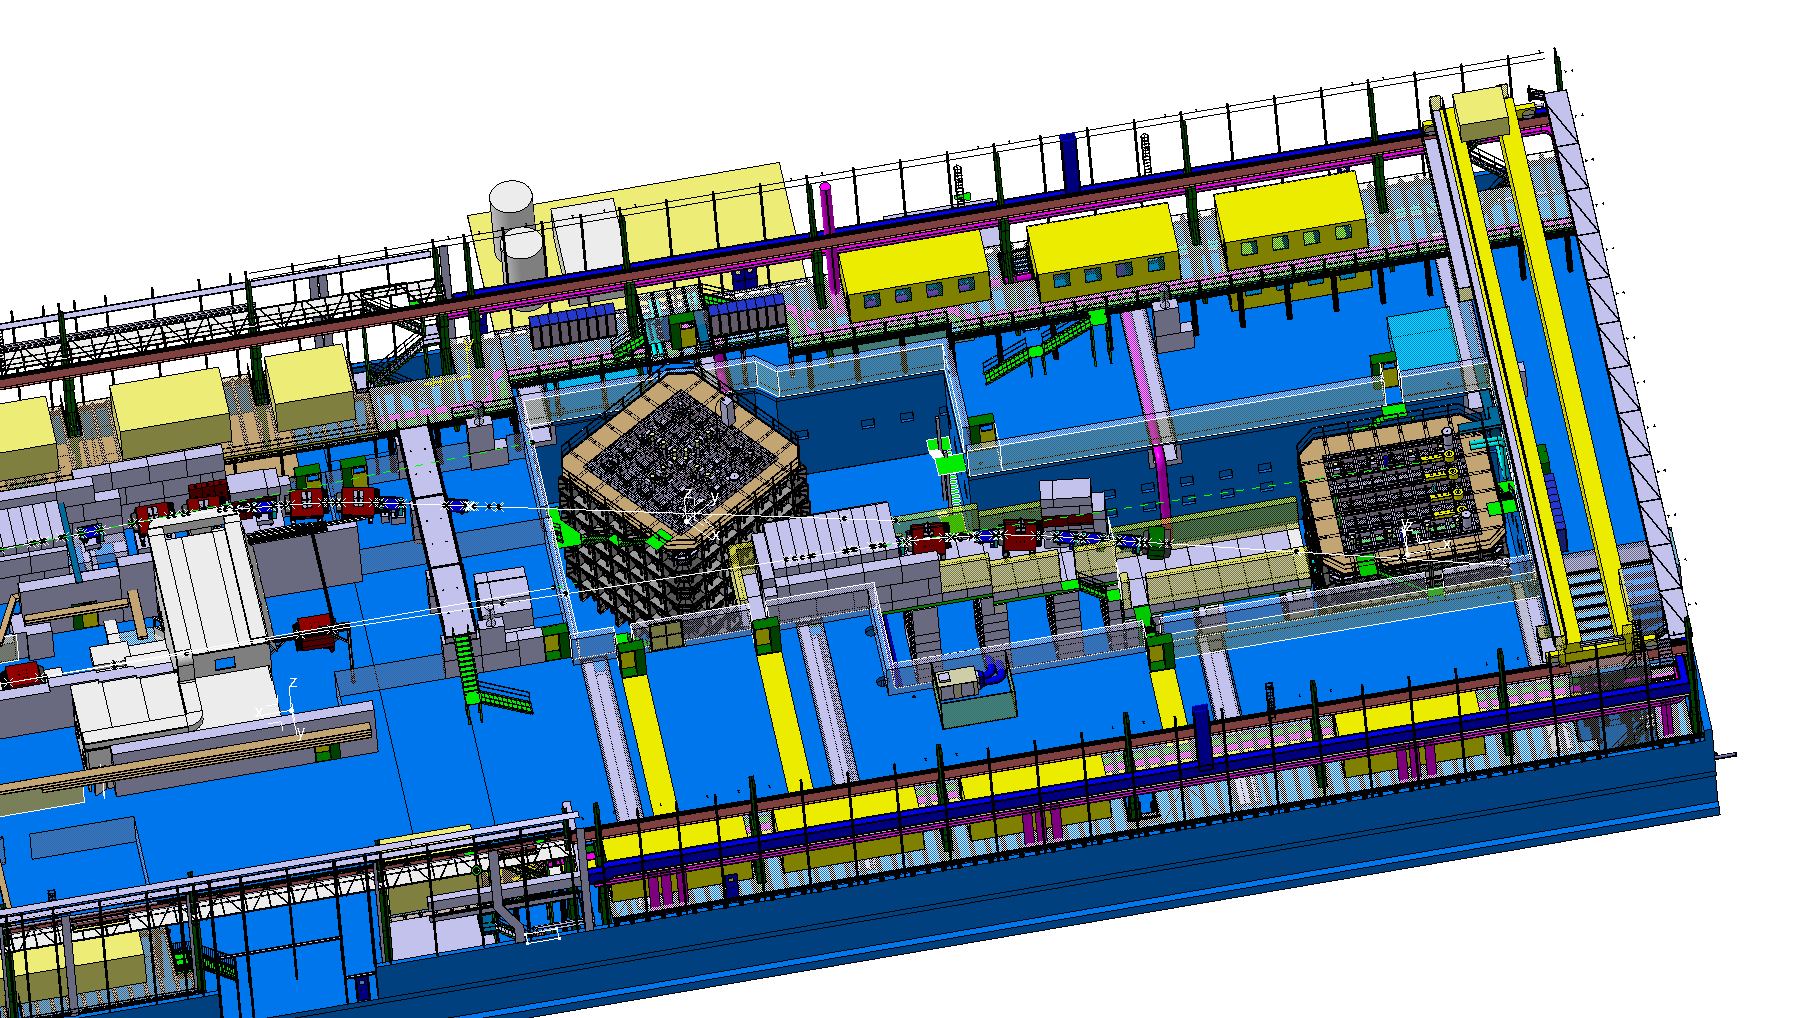
\includegraphics[width=1.0\textwidth]{np02np04.png}
\caption{\label{fig:np02np04}Diagram of the layout of the CERN north area with
  staging of the protoDUNE dual phase detector (center) and single
  phase detector (right).}
\end{figure}
%%%%%%%%%%%%%%%%%%%%%%%%

\section{Raw Data Parameters in protoDUNE-SP}
\label{sec:np04_data_rate}


\begin{table}
\begin{center}
\caption{\label{table:np04_data_rate}
  protoDUNE-SP readout parameters}
\ \\
\begin{tabularx}{0.75\textwidth}{ X  >{\setlength{\hsize}{0.8\hsize}}r}
\hline
Detector Parameter & Target \\
\hline
TPC channel count & 15,360 \\
Digitization frequency & 2\,MHz \\
Readout window & 5\,ms \\
SPS spill time& 4.8\,s\\
SPS cycle& 22.5\,s\\
Nominal trigger rate & 25\,Hz \\
Single readout size (per trigger) & 230.4\,MB \\
Lossless compression factor (estimated) & 4 \\
Instantaneous data rate (in-spill) & 1440\,MB/s \\
Average data rate & 300\,MB/s \\
Total data recorded (beam + cosmic) & 3\,PB\\
Buffer to store 3 days worth of data & 300\,TB\\
\hline
\end{tabularx}
\end{center}
\end{table}

The DUNE/\pd single-phase LArTPC design has a fine spatial resolution (with wire pitch of $\sim$\,5\,mm)
and thus a relatively high channel count. The 2\,MHz digitization provides similarly fine spatial and
temporal resolution along the drift axis of the detector. The readout window is  set to 5\,ms 
based on the nominal scale of electron drift time across the active volume (2.2\,ms).  These characteristics are typical of
similar modern TPC detectors. The principal parameters which define the expected data rate and
volume in protoDUNE-SP are presented  in Table.\,\ref{table:np04_data_rate}. In summary, combination
of the high channel count (dictated by high granularity and the volume of the detector), digitization frequency
and the relatively long readout window (due to the electron drift time) lead to a substantial data rate and volume.

\section{Data Quality Monitoring}
The protoDUNE-SP experiment will use an Online Monitoring system which will obtain data directly
from the Data Acquisition System. It is characterized by very low latency, high bandwidth and
a predefined limit on the available CPU resources (located in the vicinity of the detector). This
puts certain restrictions on what types of processing can be usefully run in this environment.

Similar to many High-Energy Physics experiments which implement ``express streams'' to
quickly conduct more detailed types of analysis in near time that can be afforded by the Online Monitoring,
protoDUNE-SP will use a prompt processing system to support Data Quality Monitoring (DQM). It will include
a few types of calculations, such as
\begin{itemize}
\item Signal Processing and basic Visualization
\item Liquid Argon purity monitoring
\item Beam Instrumentation processing and track matching
\end{itemize}

\section{Prompt Processing System}

%%%%%%%%%%%%%%%%%%%%%%%%
\begin{figure}[tb]
\centering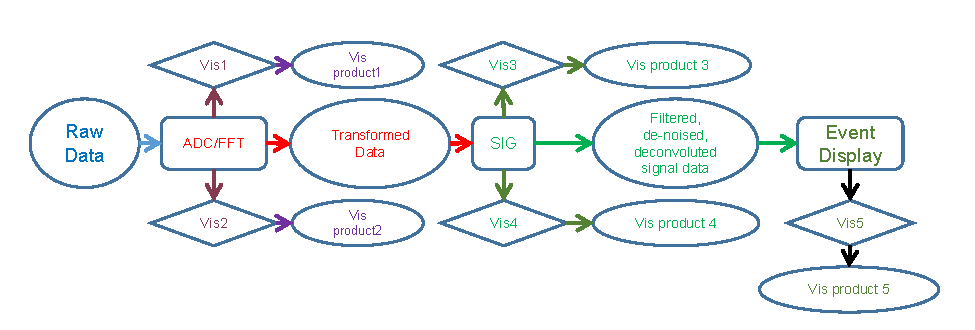
\includegraphics[width=1.0\textwidth]{dag1.pdf}
\caption{\label{fig:dag1}DAG}
\end{figure}
%%%%%%%%%%%%%%%%%%%%%%%%

\clearpage

\section*{References}
\begin{thebibliography}{9}

\bibitem{cdrVol1}
R Acciarri et al.
``Long-Baseline Neutrino Facility (LBNF) and Deep Underground Neutrino Experiment (DUNE) Conceptual Design Report Volume 1: The LBNF and DUNE Projects''.\\ e-Print: arXiv:\textbf{1601.05471}
 %DUNE CDR Vol 1 -- The LBNF and DUNE Projects.~e-Print: arXiv:1601.05471
%\url{http://arxiv.org/abs/1601.05471}

\bibitem{cdrVol4}
R Acciarri et al.
``Long-Baseline Neutrino Facility (LBNF) and Deep Underground Neutrino Experiment (DUNE) Conceptual Design Report, Volume 4 The DUNE Detectors at LBNF''.\\~e-Print: arXiv:\textbf{1601.02984}
%\url{http://arxiv.org/abs/1601.02984}

%\bibitem{np04} 
% Yearly report on ProtoDUNE Single Phase NP04 (2016), \textit{CERN-SPSC-2016-018}
%\url{https://cds.cern.ch/record/2144868}

\bibitem{xrootd}
L Bauerdick et al. ``Using Xrootd to Federate Regional Storage.'' \textit{J. Phys.: Conf. Series.} Vol.\textbf{396}. IOP Publishing, 2012.
%{XRootD software framework:}~\url{http://www.xrootd.org}

%\bibitem{cenf}
%{CERN Neutrino Platform}\\
%\url{http://home.cern/about/experiments/cern-neutrino-platform}


\bibitem{castoreos}
 L Mascetti et al. ``Disk storage at CERN.'' \textit{J. Phys.: Conf. Series.} Vol.\textbf{664}. IOP Publishing, 2015.
%{CASTOR -- CERN Advanced STORage manager}:~
%\url{http://castor.web.cern.ch/}

%\bibitem{eos}
%{The CERN Exabyte Scale Storage}\\
%\url{http://information-technology.web.cern.ch/services/eos-service}


\bibitem{sam}
R A Illingworth ``A data handling system for modern and future Fermilab experiments.''  \textit{J. Phys.: Conf. Series.} Vol.\textbf{513}. IOP Publishing, 2014.

%{A data handling system for modern and future Fermilab experiments}\\
%\url{http://iopscience.iop.org/1742-6596/513/3/032045}

\bibitem{fts}
Norman A 2014 \textit{The Fermilab File Transfer System}.~e-Print: FNAL CD-DocDB-5412
%%\url{http://cd-docdb.fnal.gov/cgi-%bin/RetrieveFile?docid=5412&filename=datamanagement-
%%changeprocedures.pdf&version=1}

\bibitem{nova}
R Plunkett et al.  ``Status of the NOvA Experiment.''  \textit{J. Phys.: Conf. Series.} Vol.\textbf{120}. IOP Publishing, 2008.


% NOvA Neutrino Experiment:~
% \url{https://www-nova.fnal.gov/}

\bibitem{uboone}
B Jones et al.  ``The Status of the MicroBooNE Experiment.''  \textit{J. Phys.: Conf. Series.} Vol.\textbf{408}. IOP Publishing, 2013.

%The MicroBooNE Experiment:~
% \url{http://www-microboone.fnal.gov/}

\bibitem{dcache}
A Millar et al.  ``dCache, agile adoption of storage technology.''  \textit{J. Phys.: Conf. Series.} Vol.\textbf{396}. IOP Publishing, 2012.
% {dCache, a distributed storage solution:}~
% \url{https://www.dcache.org/}

%\bibitem{larsoft}
%{LArSoft Collaboration}:~
%\url{http://larsoft.org//}

\end{thebibliography}



\end{document}

%%% Local Variables:
%%% mode: latex
%%% TeX-master: t
%%% End:
\grid
